%!TEX root = Main.tex
\documentclass[Main]{subfiles}

\begin{document}

\section*{Exercise 2}
Consider the function: $f:R^2 \rightarrow R, f(x) = x_1^2 + 3x_2^2 - 2x_1x_2 + 3x_2$. We wish to minize $f$ over $R^2$.
\paragraph{1: Write $f$ on the form: $\frac{1}{2} x^T Qx-x^Tb$, where $Q$ is symmetric.}


First we construct the matrix:
\\\\
$Q =$
\begin{ArgMat}
\dfrac{\partial x}{\partial x_1^2} & \dfrac{\partial x}{\partial x_1} \\
\dfrac{\partial x}{\partial x_2} & \dfrac{\partial x}{\partial x_2^2}
\end{ArgMat}
=
\begin{ArgMat}
2 & -2 \\
-2 & 6
\end{ArgMat}
\\\\
b =
\begin{ArgMat}
x_1 \\x_2
\end{ArgMat}
=
\begin{ArgMat}
0 \\ 3
\end{ArgMat}
\\\\
This gives us $\dfrac{1}{2} \cdot x^T \cdot $
\begin{ArgMat}
2 & -2 \\
-2 & 6
\end{ArgMat}
$\cdot x - x^T \cdot $
\begin{ArgMat}
0 \\ 3
\end{ArgMat}

\paragraph{2: Sketch the levels set for $f$ and the gradient of $f$ in the point $(1,1)^T$ in a $x_1x_2$-coordinate system.}

\begin{lstlisting}[caption=MatLab kode, style=Code-Matlab, label=lst:ch2-2]
[x1, x2] = meshgrid(-10:1:10, -10:1:10);
x = [x1;x2];
f1 = x1.^2 + 3*x2.^2 - 2*x1.*x2 + 3*x2;
[C,h1] = contour(x1, x2, f1, [0 3 10 50 100 200 400]);
set(h1, 'ShowText', 'on', 'TextStep', get(h1,'LevelStep') * 2)
colormap cool
title('Level sets of f(x)')
xlabel('x1')
ylabel('x2')
\end{lstlisting}

\begin{figure}[hbtp]
\centering
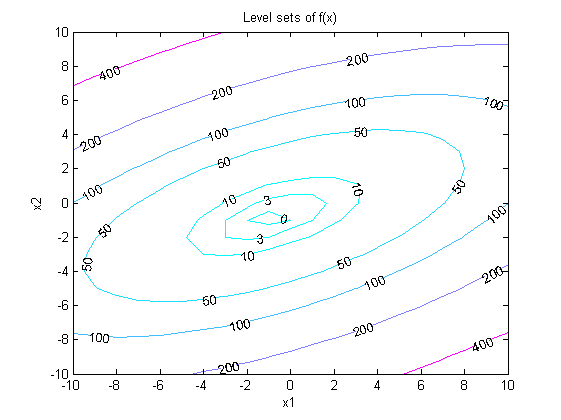
\includegraphics[width = 0.6 \textwidth]{CH2-2}
\vspace{-15pt}
\caption{Sketch of function}
\label{fig:ch2-2}
\end{figure}

The gradient can be found in $f$ in the point $(1,1)^T$ as follow:
\\
$g = Q \cdot$
\begin{ArgMat}
1 \\ 1
\end{ArgMat}
$- b = $
\begin{ArgMat}
2 & -2 \\
-2 & 6
\end{ArgMat}
$\cdot$
\begin{ArgMat}
1 \\ 1
\end{ArgMat}
$-$
\begin{ArgMat}
0 \\ 3
\end{ArgMat}
$=$
\begin{ArgMat}
0 \\ 1
\end{ArgMat}
\\
\\
\paragraph{3: Find all point satisfying the FONC. Do these points satisfy the SONC?}

FONC are found from the gradient, $f'(x) = Q \cdot x -b$, and setting it equal 0, $Q \cdot x -b = 0$.
We can solve this in \texttt{MatLab}:
\begin{lstlisting}[caption=FONC, style=Code-Matlab, label=lst:ch2-31]
Q = [2 -2;-2 6];
b = [0;3];
syms x1 x2;
X = solve(Q*[x1;x2]-b == 0)
\end{lstlisting}
$X = $
\begin{ArgMat}
\frac{3}{4} \\
\frac{3}{4}
\end{ArgMat}
\\\\
The SONC values are found by the eigens value of $Q$:
\begin{lstlisting}[caption=SONC, style=Code-Matlab, label=lst:ch2-32]
eigs(Q)
\end{lstlisting}
which yells the result 
\begin{ArgMat}
6.8284 \\
1.1716
\end{ArgMat}.
Since both are positive values the points satify the FONC.


\paragraph{4: Find the minimum of $f$ over $R^2$}
This is already found as the value $x$:
\begin{ArgMat}
\frac{3}{4} \\
\frac{3}{4}
\end{ArgMat}

\end{document}